\section{Experimental Overview}

In the next few sections of the paper, we will give detailed explanations of the experimental tasks we consider. As a preview, the tasks we consider are:

\begin{enumerate}
	\item A set of serialized objects stored externally on an HDD; the task is to read the objects into memory and deserialize them to their in-memory representation.
	\item A set of objects are stored in a large file (larger than the available RAM). The task is to perform an external sort of the file in order to perform a duplicate removal.
	\item A set of objects are partitioned across a number of machines in a network; the task is to send requests to the 	machines. Each machine answers the request by serializing the objects, then sending them over the network to the requesting machine.
	\item Finally, a set of sparse vectors are stored across various machines on a network. The task is to perform a tree aggregation where the vectors are aggregated over $log ( n )$
	hops.
\end{enumerate}

\subsection{Twitter Data Set}
For the various experiments, we use twitter data sets \cite{tweet_objects}, implemented using each of the ten different physical implementations. 

\subsection{Encoding sizes}
The ten different complex object implementations that we considered have very different encoding densities when the objects are serialized for storage or transmission across the network. The average, per-object sizes are given in Table \ref{tbl:object_size}. Figure \ref{fig:data_overview} show histogram of per objects with Standard Deviation(SD).
\begin{table}
	\centering
	\caption{Frequency of some Tweet Objects  (for 1 million tweets) }
	\label{tbl:object_size}
	\begin{adjustbox}{width=\columnwidth,center}	
		
		\begin{tabular}{|c|c|c|l|} \hline
			Object Name &Parent Object &Frequency&AVG Size(byte)\\ \hline
			tweet  & root object& 1,000,000 & 6599.305602\\ \hline
			users & tweet & 1,000,000 & 1453.798722\\ \hline
			coordinates  &tweet& 1586 & 57.87705\\ \hline
			place & tweet & 11974 & 392.8976115\\ \hline
			quoted status  & tweet & 177537 & 3993.947594\\ \hline
			retweeted status  & tweet & 598517 & 4775.996797\\ \hline
			entities  & tweet & 1,000,000 &336.02128\\ \hline
			extended entities  & tweet & 51479 & 1133.00505\\ \hline
			hashtags  & entities & 398720 & 44.0340615\\ \hline
			media  & entities & 51481 & 762.556516\\ \hline
			urls  & entities & 417176 & 187.6829563\\ \hline
			user mentions  & entities & 1063216 & 126.845482\\ \hline
			symbols  & entities & 7793 & 36.55832\\ \hline
			sizes  & media & 7793 & 36.55832\\ \hline
			media sizes  & sizes & 51485 & 194.91743\\ \hline
			thumb  & media sizes & 51485 & 37.989\\ \hline
			large  & media sizes & 51485 & 37.524\\ \hline
			medium  & media sizes & 51485 & 37.412\\ \hline
			small  & media sizes & 51485 & 36.993\\ \hline
			\hline\end{tabular}
	\end{adjustbox}
\end{table}

\begin{figure*}
	\centering
	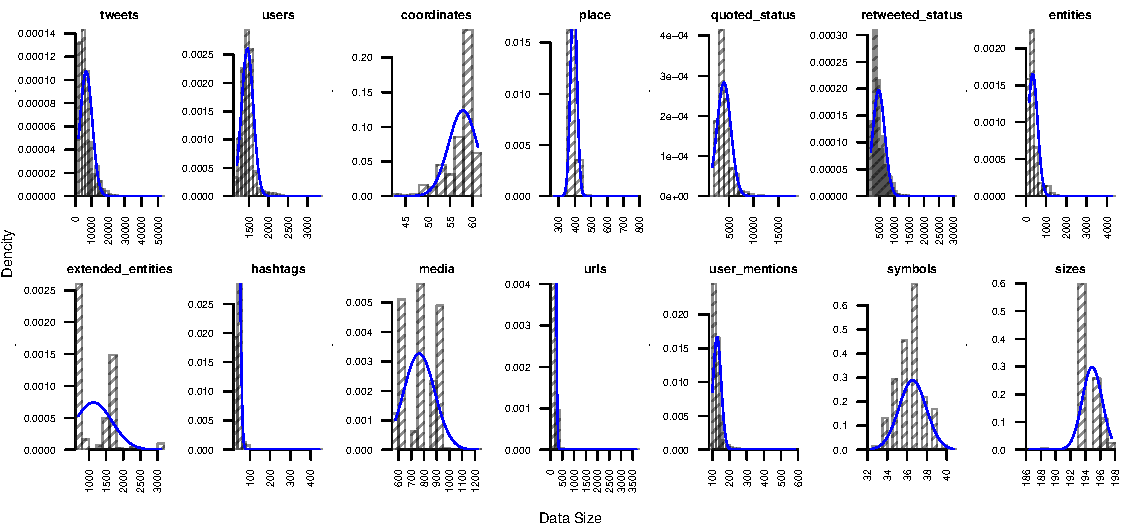
\includegraphics[scale=1]{img/Data_Overview.pdf}
	\caption{histograms with Standard Deviation}
	\label{fig:data_overview}
\end{figure*}

\subsection{Experimental Details}
We run our experiments on a virtual server instances which have 8 vCPU cores, 32 GB RAM and one 800
GB hard disks (Network Instance Store) running with Ubuntu 18.04.3 LTS. Before running each experiment task, we “warmed up” the Java Garbage Collector (GC) by creating a large number of objects. We do not include this warm-up-time in our performance time calculations.

We used two Java GC flags $-XX:-UseGCOverheadLimit$ and $-XX:+UseConcMarkSweepGC$. The first flag is used to avoid OutOfMemoryError exceptions while using the complete RAM size for data processing and the second flag is for running concurrent garbage collection.

We run all of our experiments 5 times and observed that the results have low variance. In this paper we present the average of those runs. Before running each experiment, we
deleted th OS cache using the Linux command: $echo 3 > /proc/sys/vm/drop_caches$.

Our Java implementation is written using Java 8 with the Oracle JDK version "1.8.0\_241" and for our C++ implementation we use the C++11, compiled using clang++ (version 6.0.0).

The source codes of our implementation and a brief description of technical details can be found on the Github Repository \footnote{The source code of our Implementation is available at \url{https://github.com/fathollahzadeh/serialization}} .
